\section{Der „neue Mensch“ und die Technisierung des Haushalts}

\subsection{Einführung: Rationalisierung als gesellschaftliches Leitbild}

Die Vorlesung untersucht die Ausweitung technischer und wissenschaftlicher
Rationalisierung auf immer neue Bereiche des gesellschaftlichen Lebens.

Während Rationalisierung zunächst vor allem mit industrieller Produktion
verbunden war, entstand im Verlauf des 19. und 20. Jahrhunderts die Vorstellung,
dass auch Menschen, Lebensweisen und soziale Strukturen
wissenschaftlich gestaltet und optimiert werden könnten.

Grundlage dafür war ein tiefes Vertrauen in Wissenschaft,
Technik und Fortschritt.

Diese galten als objektive Instrumente,
mit deren Hilfe sich gesellschaftliche Probleme lösen
und die Lebensbedingungen verbessern liessen.

Zentrale Leitfragen:

\begin{itemize}
    \item Wie wurde der Mensch selbst zum Gegenstand technischer Planung?
    \item Welche Vorstellungen von Fortschritt prägten das 20. Jahrhundert?
    \item Wie beeinflussten Wissenschaft und Technik Alltag und Lebensführung?
    \item Weshalb wurde auch der Haushalt rationalisiert?
\end{itemize}

Die Geschichte der Technisierung des Haushalts ist daher nicht nur
Technikgeschichte, sondern auch Sozial-, Kultur- und Ideengeschichte.

\subsection{Industrialisierungserfahrungen und die Idee der gesellschaftlichen Optimierung}

Die Industrialisierung führte nicht nur zu wirtschaftlichen Veränderungen,
sondern auch zu neuen gesellschaftspolitischen Vorstellungen.

Viele Reformbewegungen gingen davon aus,
dass Wissenschaft und Technik genutzt werden könnten,
um Individuen und Gesellschaft gezielt zu verbessern.

Zu den wichtigsten Strömungen gehörten:

\begin{itemize}
    \item Eugenik
    \item Lebensreform
    \item die Vorstellung des „neuen Menschen“
\end{itemize}

Obwohl sich diese Bewegungen stark unterschieden,
teilten sie die Annahme,
dass gesellschaftlicher Fortschritt durch Planung,
Steuerung und Optimierung erreicht werden könne.

\subsection{Eugenik und die wissenschaftliche Steuerung des Menschen}

Die Eugenik verstand sich als wissenschaftlich begründetes Programm
zur Verbesserung der Gesellschaft durch die Kontrolle menschlicher Fortpflanzung.

Typische Massnahmen waren:

\begin{itemize}
    \item Eheverbote
    \item Zwangssterilisationen
    \item Gesundheits- und Hygienekampagnen
    \item Förderung bestimmter Bevölkerungsgruppen
\end{itemize}

Die Eugenik verband Wissenschaft,
Politik und Moral zu einem System gesellschaftlicher Steuerung.

Ziel war die Schaffung eines gesunden,
leistungsfähigen und produktiven „Volkskörpers“.

Heute gilt die Eugenik als Beispiel dafür,
wie wissenschaftliche Autorität zur Legitimation
von Diskriminierung und Gewalt eingesetzt werden konnte.

\begin{center}
    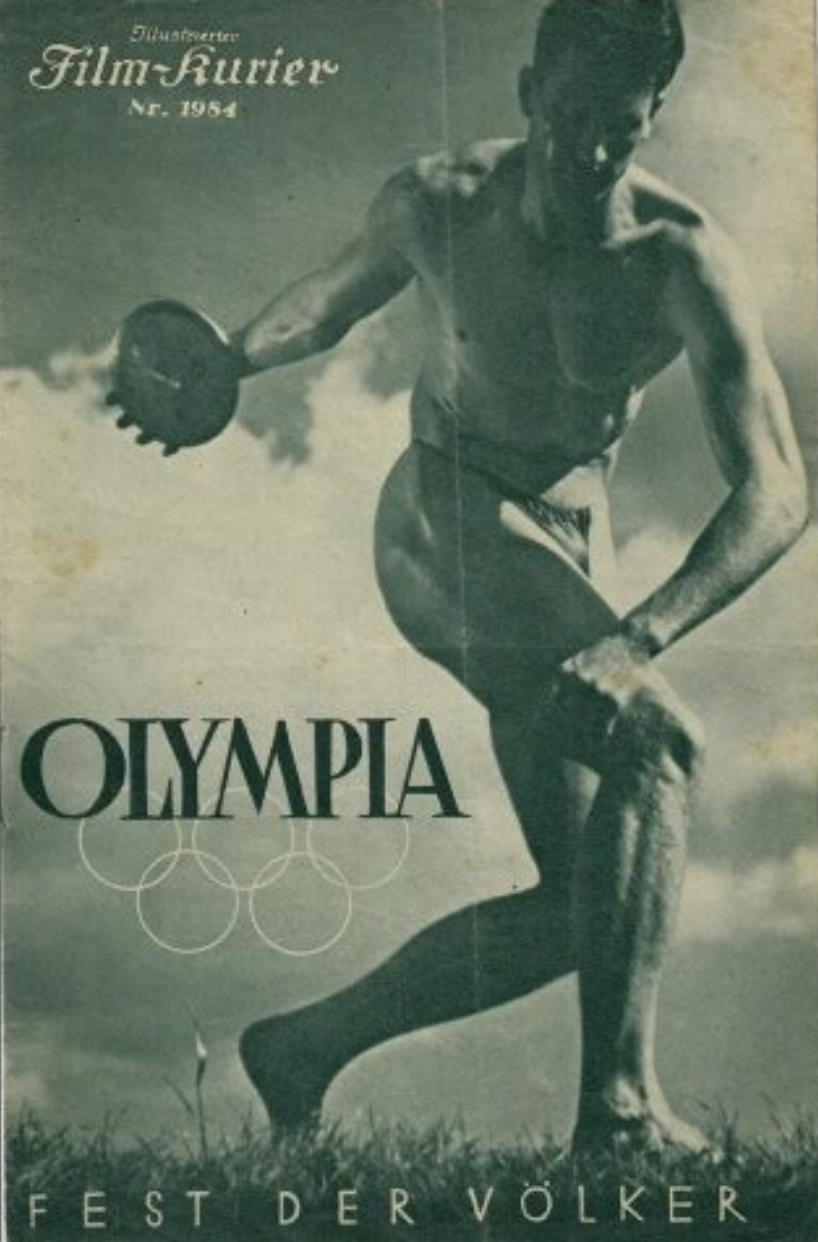
\includegraphics[width=0.55\linewidth]{images/olympia_1936.png}
\end{center}

\subsection{Lebensreform und die Suche nach dem natürlichen Leben}

Parallel zur Eugenik entwickelte sich die Lebensreformbewegung.

Sie kritisierte die Folgen von Industrialisierung,
Urbanisierung und Massenkonsum.

Angestrebt wurden:

\begin{itemize}
    \item gesunde Ernährung
    \item Körperkultur und Sport
    \item Naturheilkunde
    \item naturnahe Lebensformen
\end{itemize}

Die Bewegung verstand sich als Gegenentwurf
zur modernen Industriegesellschaft.

Gleichzeitig beruhte auch sie auf der Vorstellung,
dass Menschen und Gesellschaft gezielt verbessert
und optimiert werden könnten.

Dadurch weist sie trotz ihrer Kritik an der Moderne
Parallelen zu anderen Rationalisierungsprojekten auf.

\begin{center}
    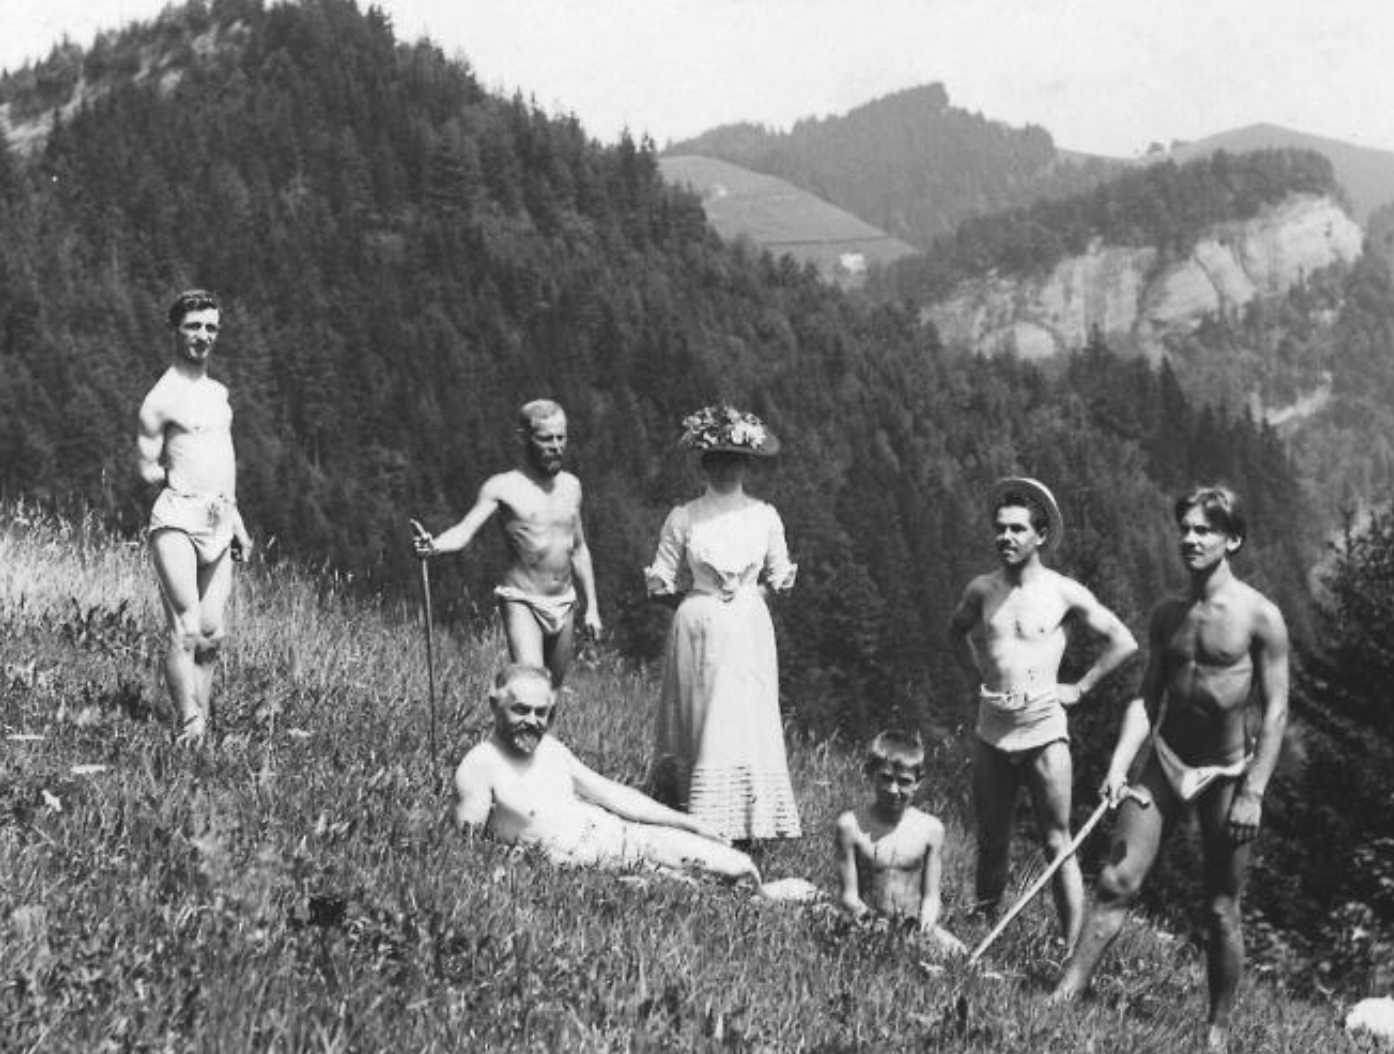
\includegraphics[width=0.8\linewidth]{images/monte_verita.png}
\end{center}

\subsection{Der „neue Mensch“ als gesellschaftliches Ideal}

Besonders im sozialistischen Denken entstand die Vorstellung
eines „neuen Menschen“.

Dieser sollte nicht nur technisch ausgebildet,
sondern auch moralisch, sozial und politisch
den Anforderungen einer zukünftigen Gesellschaft entsprechen.

Dazu dienten unter anderem:

\begin{itemize}
    \item Bildung und Erziehung
    \item Gesundheitsprogramme
    \item Arbeitsorganisation
    \item Freizeit- und Kulturangebote
\end{itemize}

Technischer Fortschritt,
gesellschaftlicher Fortschritt und moralische Entwicklung
wurden dabei als untrennbare Einheit verstanden.

Die Optimierung des Menschen galt zugleich
als Optimierung der Gesellschaft.

\begin{center}
    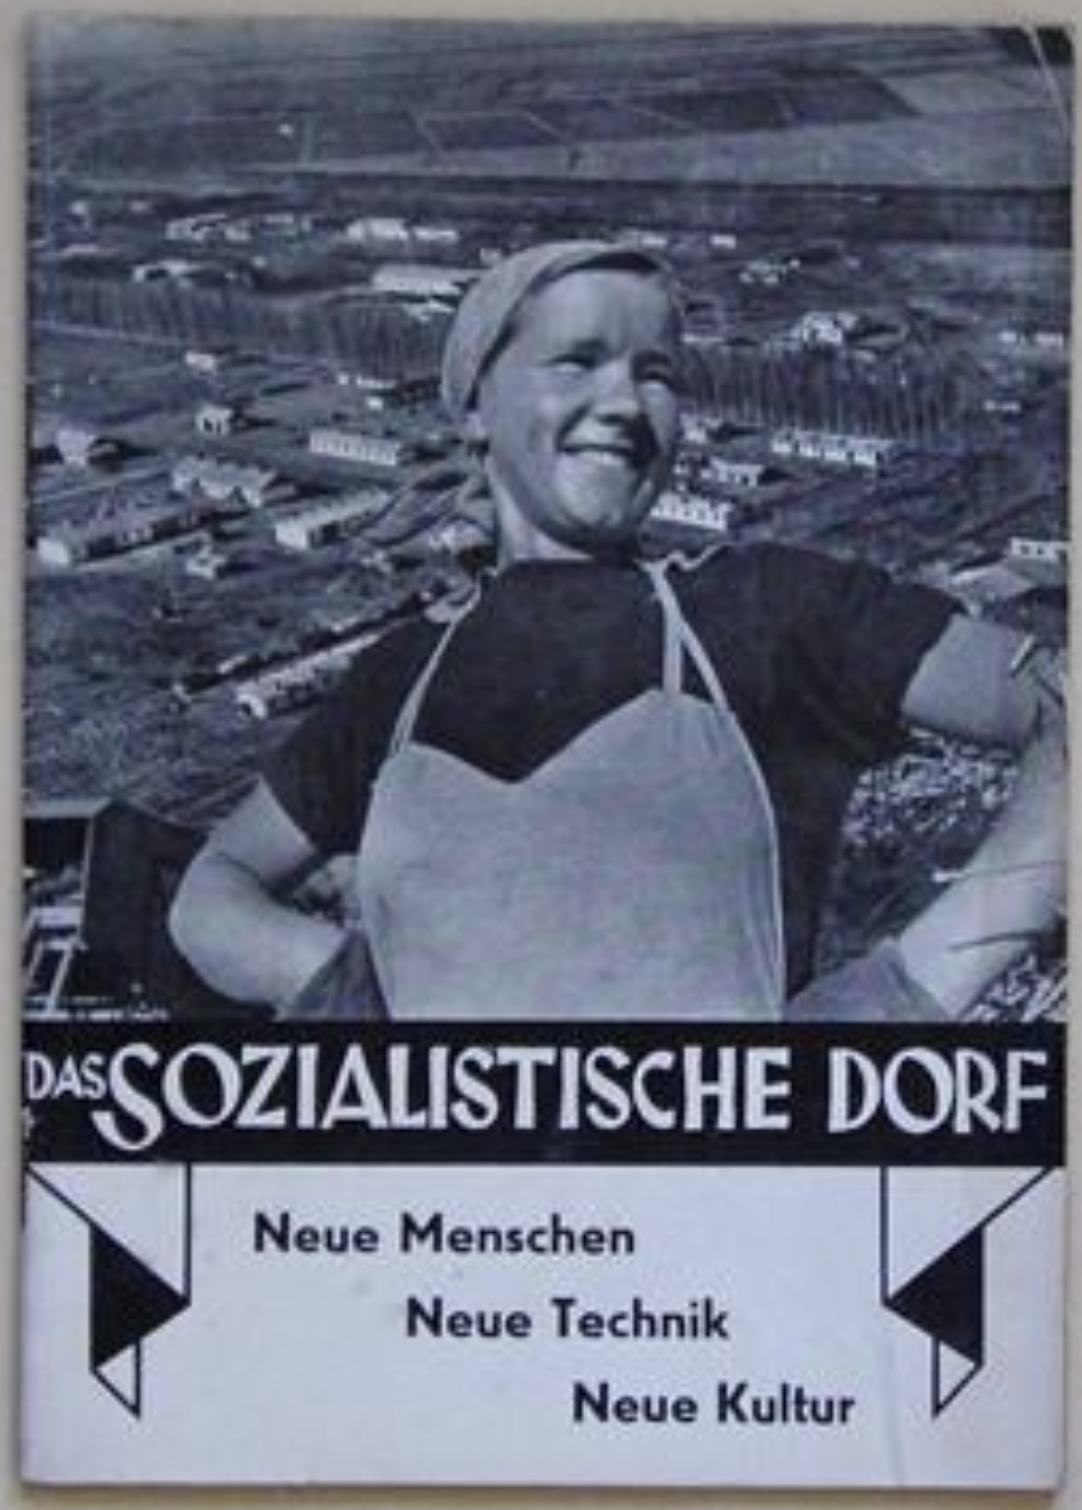
\includegraphics[width=0.55\linewidth]{images/sozialistisches_dorf.png}
\end{center}

\subsection{Technik, Wissenschaft und soziale Kontrolle}

Die Vorlesung zeigt,
dass Wissenschaft und Technik im 20. Jahrhundert
zunehmend als Instrumente gesellschaftlicher Steuerung eingesetzt wurden.

Menschen wurden vermessen,
klassifiziert und analysiert.

Dazu gehörten:

\begin{itemize}
    \item Körperstudien
    \item Bewegungsanalysen
    \item Leistungsmessungen
    \item medizinische und genetische Untersuchungen
\end{itemize}

Wissenschaftliche Erkenntnisse erschienen dadurch objektiv und neutral.

Tatsächlich waren sie jedoch häufig eng mit politischen,
gesellschaftlichen und moralischen Zielvorstellungen verbunden.

Technik strukturierte Verhalten zunehmend,
ohne dass direkter Zwang notwendig war.

\subsection{Rationalisierung des Wohnens}

Die Prinzipien der Rationalisierung beschränkten sich nicht auf Fabriken.

Auch Wohnräume wurden zum Gegenstand technischer Planung.

Ausgangspunkt waren:

\begin{itemize}
    \item Wohnungsnot
    \item Verstädterung
    \item neue Vorstellungen von Hygiene
    \item funktionale Architektur
\end{itemize}

Die Architektur der Neuen Sachlichkeit
forderte zweckmässige und effizient gestaltete Wohnungen.

Wohnräume wurden neu organisiert,
Arbeitsabläufe vereinfacht
und traditionelle Wohnformen verändert.

\begin{center}
    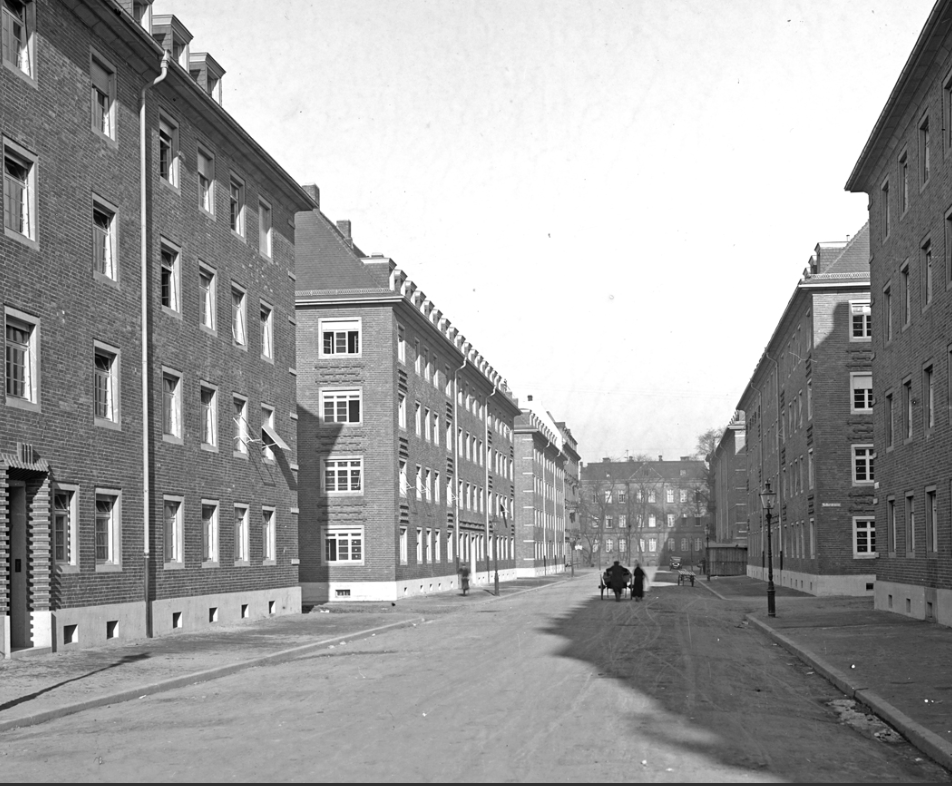
\includegraphics[width=0.85\linewidth]{images/wohnungsnot_moderner_wohnblock.png}
\end{center}

\subsection{Die Frankfurter Küche}

Ein besonders bekanntes Beispiel
für die Rationalisierung des Alltags
ist die Frankfurter Küche von Margarete Schütte-Lihotzky.

Sie wurde ab 1926 entwickelt
und orientierte sich an den Prinzipien
wissenschaftlicher Arbeitsorganisation.

Ziel war die Reduktion unnötiger Wege
und die Effizienzsteigerung der Hausarbeit.

Die Küche wurde als funktionaler Arbeitsraum gestaltet,
dessen Aufbau auf Bewegungsanalysen beruhte.

Damit übertrug man die Logik industrieller Rationalisierung
auf den privaten Haushalt.

\begin{center}
    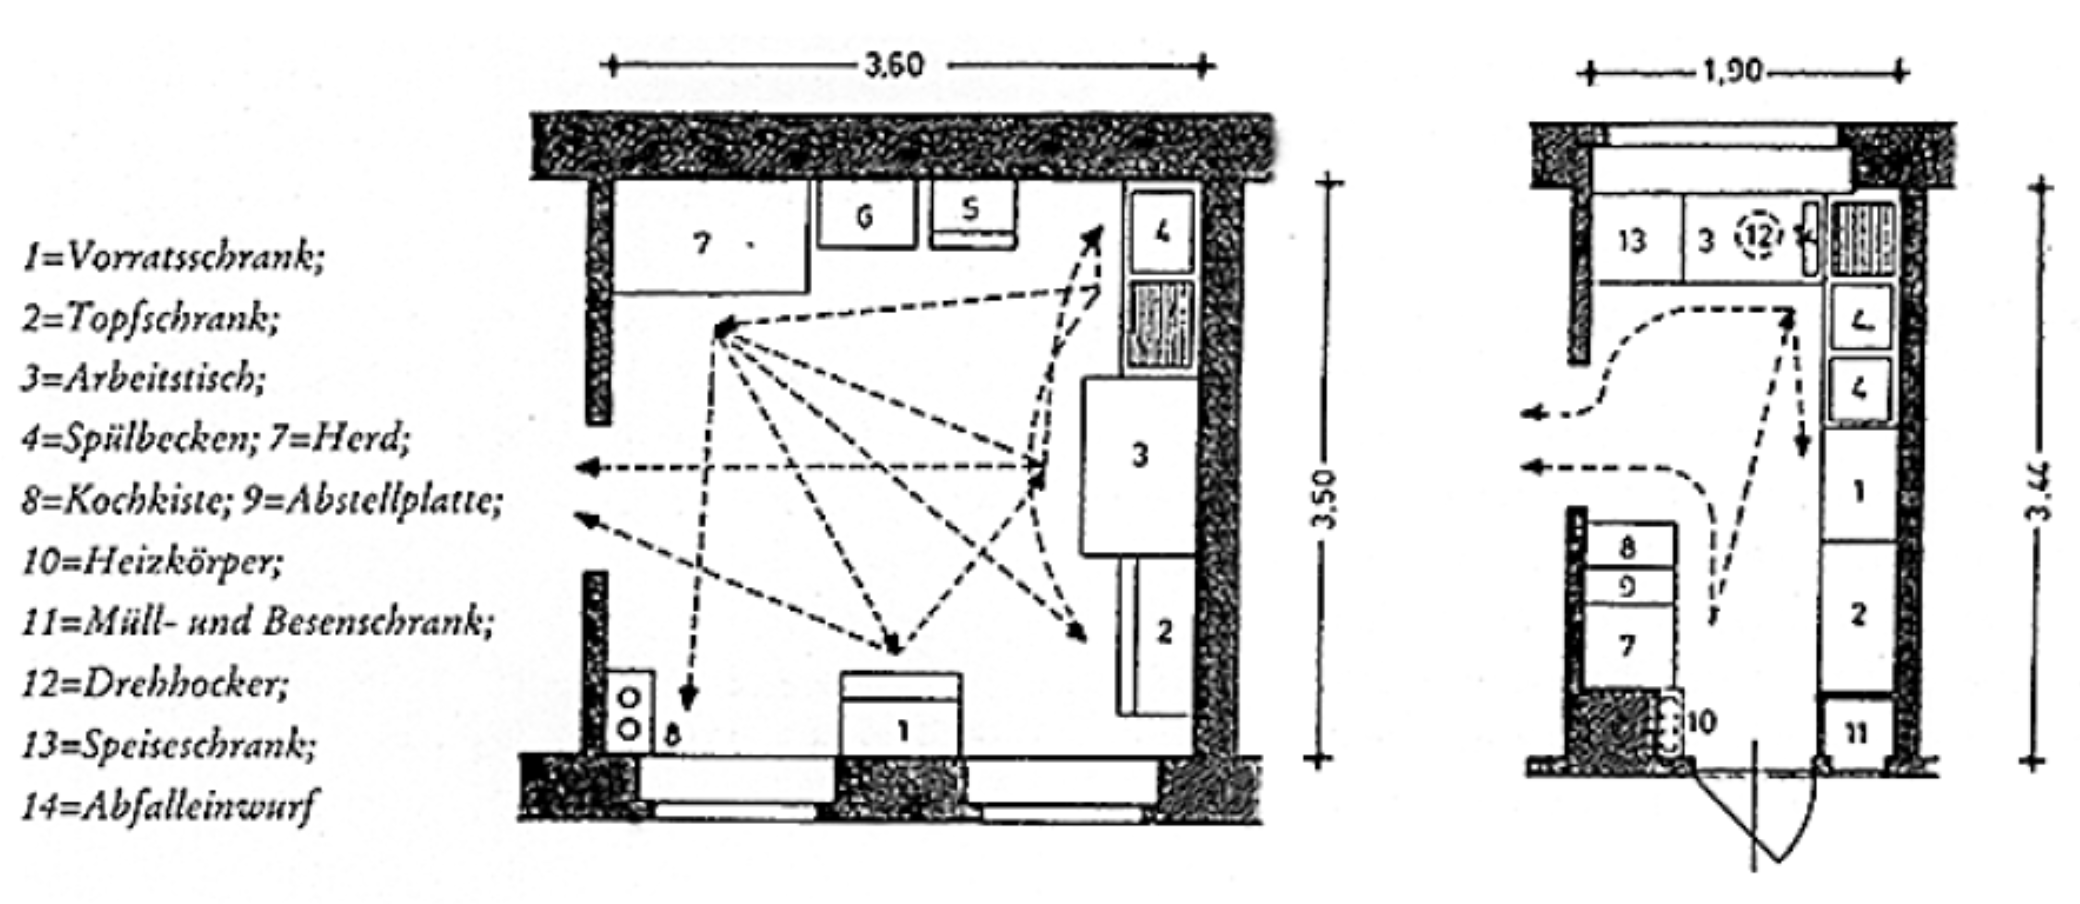
\includegraphics[width=0.9\linewidth]{images/frankfurter_kueche.png}
\end{center}

\subsection{Emanzipation und Kontrolle}

Die Rationalisierung des Alltags besitzt eine doppelte Bedeutung.

Einerseits versprach sie:

\begin{itemize}
    \item höheren Lebensstandard
    \item bessere Hygiene
    \item gesundheitliche Verbesserungen
    \item Arbeitserleichterungen
\end{itemize}

Andererseits führte sie zu neuen Formen
gesellschaftlicher Kontrolle und Normierung.

Die Soziologen Max Horkheimer und Theodor W. Adorno
kritisierten diese Entwicklung als „instrumentelle Vernunft“.

Sie warnten davor,
dass Rationalität zunehmend zum Instrument
der Kontrolle von Menschen und Gesellschaft werde.

Die Geschichte der Technisierung des Haushalts
bewegt sich daher stets im Spannungsfeld
zwischen Befreiung und Kontrolle.

\subsection{Zentrale Erkenntnisse}

Die Vorlesung zeigt,
dass technische Rationalisierung weit über Fabriken hinauswirkte.

Sie beeinflusste:

\begin{itemize}
    \item Vorstellungen von Gesundheit
    \item Erziehung und Bildung
    \item Wohnformen
    \item Haushaltsführung
    \item gesellschaftliche Normen
\end{itemize}

Die zentrale These lautet:

Die Technisierung des Haushalts ist Teil eines umfassenden historischen Prozesses,
in dem Wissenschaft und Technik nicht nur Maschinen,
sondern auch Menschen, Lebensweisen und soziale Strukturen
gestalten sollten.

Dabei entstanden sowohl neue Freiheiten
als auch neue Formen gesellschaftlicher Kontrolle.